\chapter{Scalability}
\label{chap:Scalability}

Graph visualizations are always limited by the number of nodes, as well as the number of edges. The patterns in figure \ref{fig:patterns} can only be recognised if completely visible, therefore the hole adjacency matrix must be visible to find all of them. Otherwise patterns may not be entirely visible. This chapter gives an overview of the scalability of adjacency matrices, by estimating the upper limit of nodes in full visible adjacency matrix visualisations, explaining the problems of non full visible matrix visualisations, and reviewing the implementations 'Matrix zoom' \citep{ham-ivis-2003, abello} and Nodetrix \citep{henry}.


\section{Maximum number of nodes in full visible adjacency matrices}
A short best case estimation will show the scalability limits of full visible adjacency matrix visualisations. Assuming all patterns should be recognisable, the hole matrix must be visible at once. Given a screen size of 25”, the number of nodes depends on the size of column, row and cell size. The number of displayable edges is in adjacency matrixes is always $|nodes|^2$.

Size of cells, rows and columns is determined by the their requirements. Pure visibility, intractability, or permanent visible node labels, or edge weights (cell labels) require increasingly more space.
If only a visible mark is required for an edge, a pixel is the lower limit for the marks size, otherwise marks can not be associated to the source or destination edge. Hi resolution screens do not increase the maximum number of nodes, since it is getting very hard to follow the grid lines to other nodes. By the way: my dsit trauma wants me to calculate the entropy of such matrix instance. Anyway, more than ~3000 nodes on a screen will cause a unreadable visualisation.
Mouse interactions like ‘on hover tooltips’ will add the option to identify source and destination nodes of an edge, but will also use more space and restrict the max nr of nodes. This will shrink the maximum number of nodes to ~300.
If edge node assoziation is an important task, permanent visible node labels in header will allow a interaction less visualisation of the graph. Additional space for labels reduces the maximum node number to 30.
 
 
\begin{table}[]
\centering
\begin{tabular}{|l|l|l|}
\hline
25" screen                 & max nodes & max edges                \\ \hline
Pixel grid                 & 3000      & $10^7$                     \\ \hline
Interactive cell or header & 300       & $10^5$                     \\ \hline
Labeled cell or header     & 30        & $10^3$                     \\ \hline
\end{tabular}
\caption{My caption}
\label{my-label}
\end{table}



\section{Non full visible adjacency matrices - zooming}
Putting a adjacency matrix in a zoom box obviously increases the maximum number nodes. 
When zoomed in, the readability of node and cell labels increases, but patterns may not be completely visible anymore. This requires the user to search the matrix by panning, a lot of panning. When zoomed out, labels are not readable anymore, and interactions with cells are impossible due to their small size. 

The following two section reviews Matrix zoom, a zoomable matrix visualisation which is avoiding these problems for clustered graphs. A general solution, without using known additional properties of the graph like the its clusters, was not found in the survey.

\section{Matrix subdivision}

Matrix zoom is a zoomable matrix visualisation [\cite{ham-ivis-2003}. It solves the label readability problem by finding new labels for groups of nodes or edges when zoomed out. It comes with a default dataset, describing a software repository. The nodes of the actual graph are function declarations and function calls of the source code, so it is the complete call graph of a software project. Classes, packages and layers are considered as clusters of the graph. 

When node labels get too small to read, they form groups by their containing classes, these groups are labeled with the class name. Multiple classes are represented by packages and so on. When edge marks get too small, a $n \times m$ block of edge marks is transformed to one cell, by calculating the density of the block and associating the cell color to to it.

\begin{figure}[h]
\centering
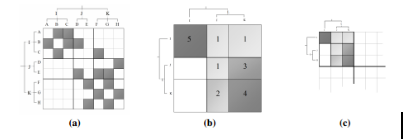
\includegraphics{images/matrixzoom_transform}
\caption{Cell and header transformations \citep{ham-ivis-2003} \label{fig:matrixzoom_transform}}
\end{figure}




\subsection{Cell and header transformations}   
This concept needs in general a way to transform blocks of labels to one label. The given example fits well to this requirement, since classes, packages are clusters and have human readable names. If the graph is clustered by algorithms, meaningful names of clusters must be found, see figure \ref{fig:matrixzoom_transform}.

If other header visualisation techniques are used, the transformation must be adopted, see Capter \ref{chap:headers}. For example if in or out degrees are visualized in the header, the average degree might be visualized by the group.

Transforming cell blocks to a cell can be done in various ways. If just the existence of an edge is relevant, the group cell may be rendered like a edge if at least one edge is in the cluster. Average weight, density or degree may also be relevant. Which of this transformations should be used is dependent on the requirements of the application, however, only one can be chosen.

This concept is suitable for recursive clustering, where each cluster is a zoom level. [Abello] shows an extended version of Matrix zoom using tree structures in the matrix headers for better navigation, see figure \ref{fig:matrixzoom_abello}.

\begin{figure}[h]
\centering
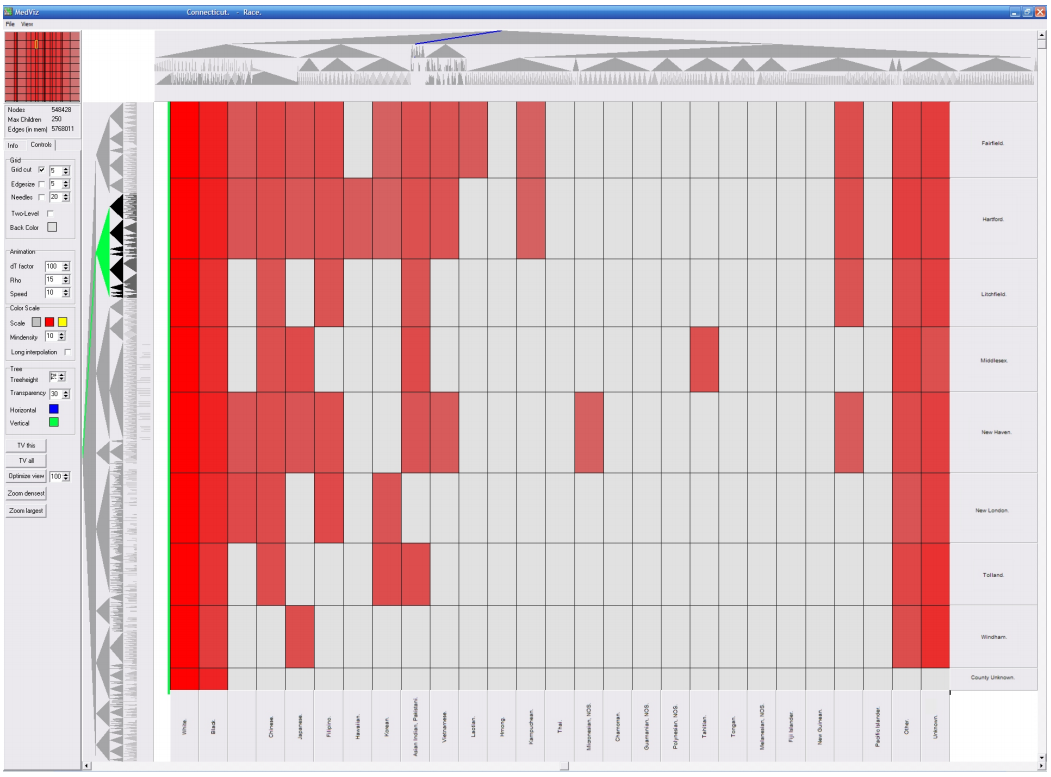
\includegraphics[width=\textwidth]{images/matrixzoom_abello}
\caption{Cluster tree visualised as in matrix header for better navigation \citep{abello} \label{fig:matrixzoom_abello}}
\end{figure}





\subsection{Sorting and clustering}   

The ‘edge mark in invisible area' problem is reduced by the clustering, since most connections are within the cluster, it is less likely to have invisible edge marks if zoomed to a cluster. See figure \ref{fig:matrixzoom_cluster}. 
The quality of this reduction depends on the chosen cluster algorithm, and the sort algorithm, see figure \ref{fig:reorder}. In general the cluster algorithm is execued first, and the order argorthm is applyed to the elements within the cluster, and then to the clusters them self.

\begin{figure}[h]
\centering
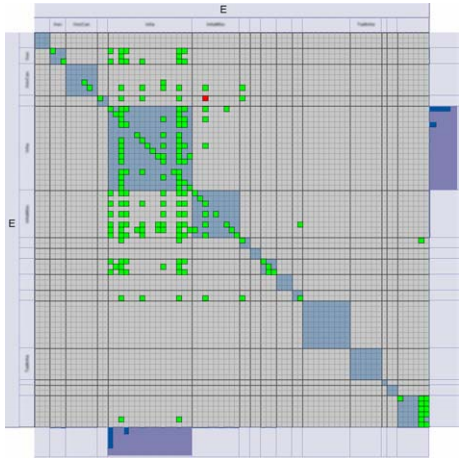
\includegraphics[width=\textwidth/2]{images/matrixzoom_cluster}
\caption{Typical matrix subdivision view of Matrix zoom\citep{ham_phd} \label{fig:matrixzoom_cluster}}
\end{figure}

This concept can not be applied always. In best case the dataset gives a natural cluster tree like the software repository, otherwise suitable cluster algorithm must be found, as well as human readable labels for those automatically generated clusters. In should be considered as data preprocessing, since it may be applied to large datasets.













\section{Hybrid Representation}
Nodetrix is a graph adjacency matrix hybrid. Adjacency matrices are better suited for dense graphs, so the idea of nodetrix is, to replace unreadable dense subclusters in traditional graph visualisations with adjacency matrix visualisations. Figure \ref{fig:nodetrix_cluster} shows a traditional graph, with a dense green cluster. It is hard to find the nodes of a edge in the traditional view on the left. On the right side the dense subcluster is replaced by a better readable  adjacency matrix. Edges out of the cluster are rendered als lines to the nodes in the traditional graph view, or other matrix views, and therefore always visible \citep{henry-nodetrix-2007}.



\begin{figure}[h]
\centering
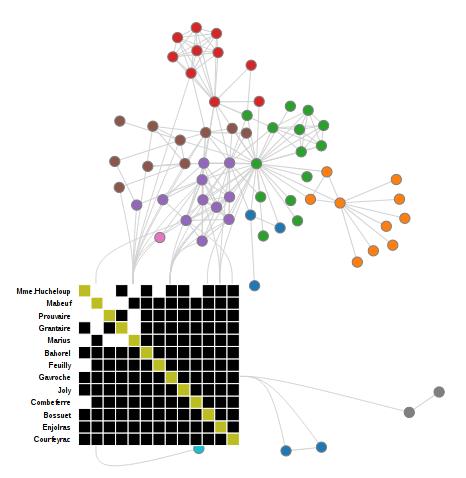
\includegraphics[width=\textwidth/3]{images/nodetrix_cluster}
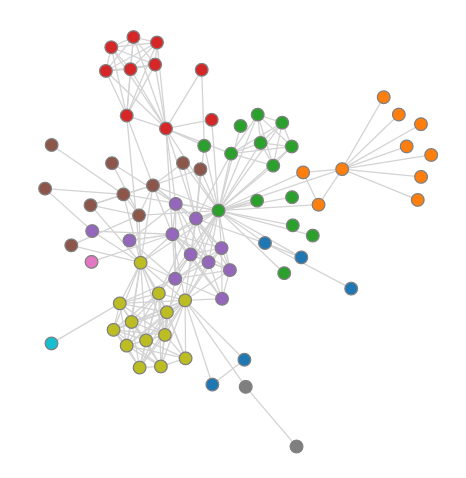
\includegraphics[width=\textwidth/3]{images/nodetrix_matrix}
\caption{Typical matrix subdivision view of Matrix zoom\citep{henry-nodetrix-2007} \label{fig:nodetrix_cluster}}
\end{figure}
